\documentclass{beamer}
\usepackage[utf8]{inputenc}
\usepackage[T1]{fontenc}
\usepackage{graphicx}
\usepackage{tcolorbox}
\usepackage{hyperref}
\hypersetup{
    colorlinks=true,
    linkcolor=pink,
    urlcolor=cyan,
    urlbordercolor=cyan,
}
\graphicspath{ {./images/} }

\usetheme{Arguelles}

\title{Tutorial 7}
\subtitle{CS3241 Computer Graphics (AY22/23)}
\date{\today}
\author{Wong Pei Xian}
\institute[]{\email{e0389023@u.nus.edu}}

\begin{document}

\frame[plain]{\titlepage}

\section{Recap}

\begin{frame}[plain,standout]
    prepare \url{pollev.com/peixian} for later
\end{frame}

\begin{frame}[plain,standout]
    \AlegreyaExtraBold \LARGE
    Recap of Texture Mapping
\end{frame}

\begin{frame}
    \frametitle{Texture Mapping}

    \begin{itemize}
        \item One of the most foreign parts of graphics programming
        \item Many parameters and states for \textbf{fragment processing}
        \begin{itemize}
            \item Texture magnification
            \item Mipmapping (texture minification)
            \item Framebuffer data
            \item Texture environments
        \end{itemize}
    \end{itemize}

\end{frame}

\begin{frame}
    \frametitle{Local parameters (Bound texture)}

    \begin{center}
        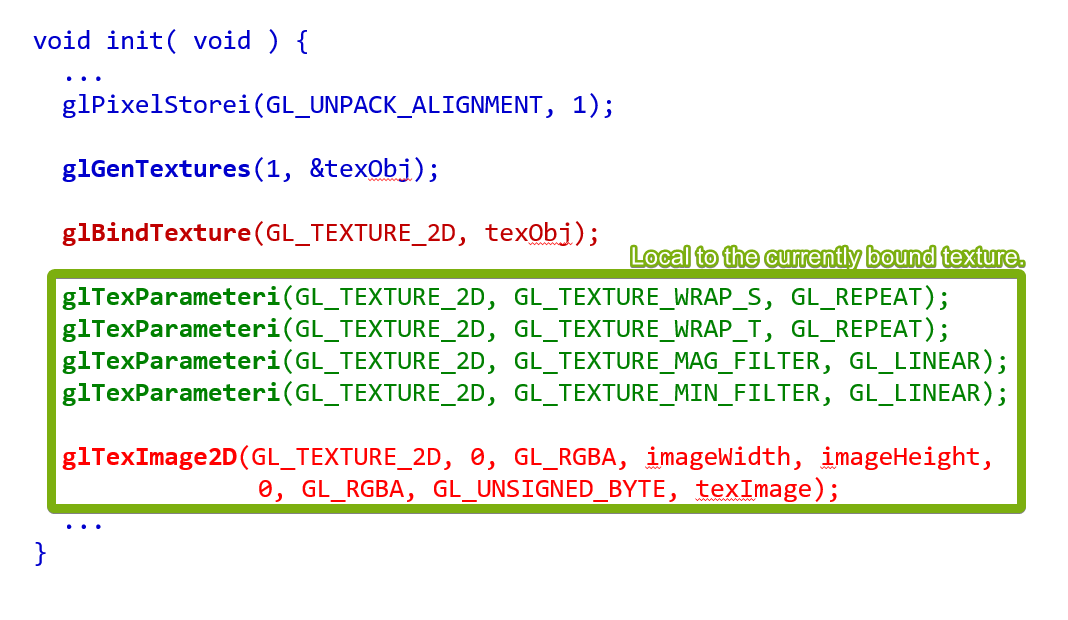
\includegraphics[scale=0.5]{local-bound-texture.png}
    \end{center}

\end{frame}

\begin{frame}
    \frametitle{Global state (Texture Environment)}

    \begin{center}
        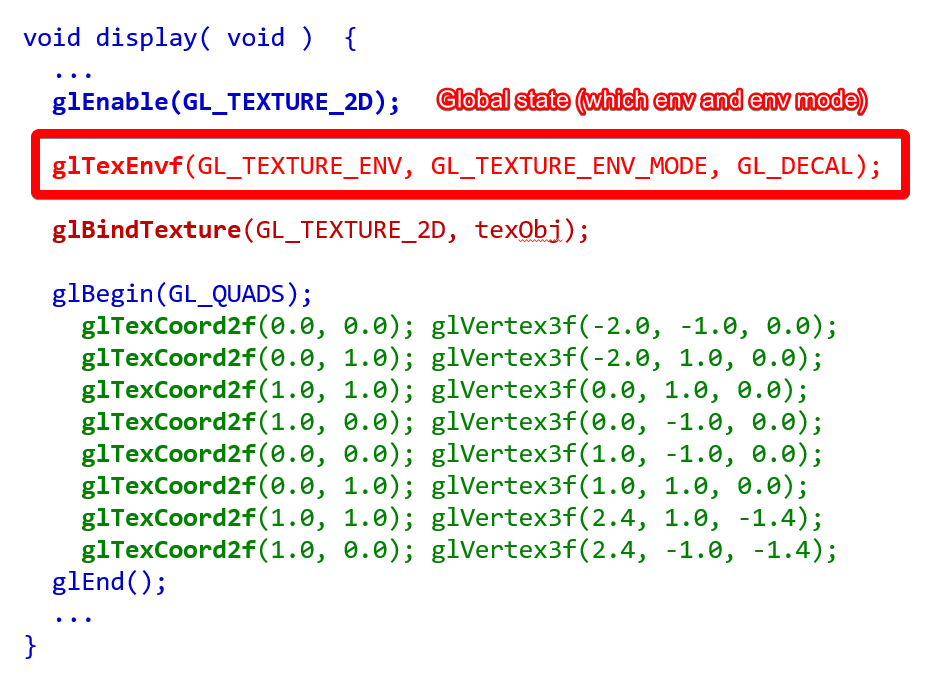
\includegraphics[scale=0.5]{global-vars.png}
    \end{center}

\end{frame}

\begin{frame}
    \frametitle{Texture Environments}

    \begin{center}
        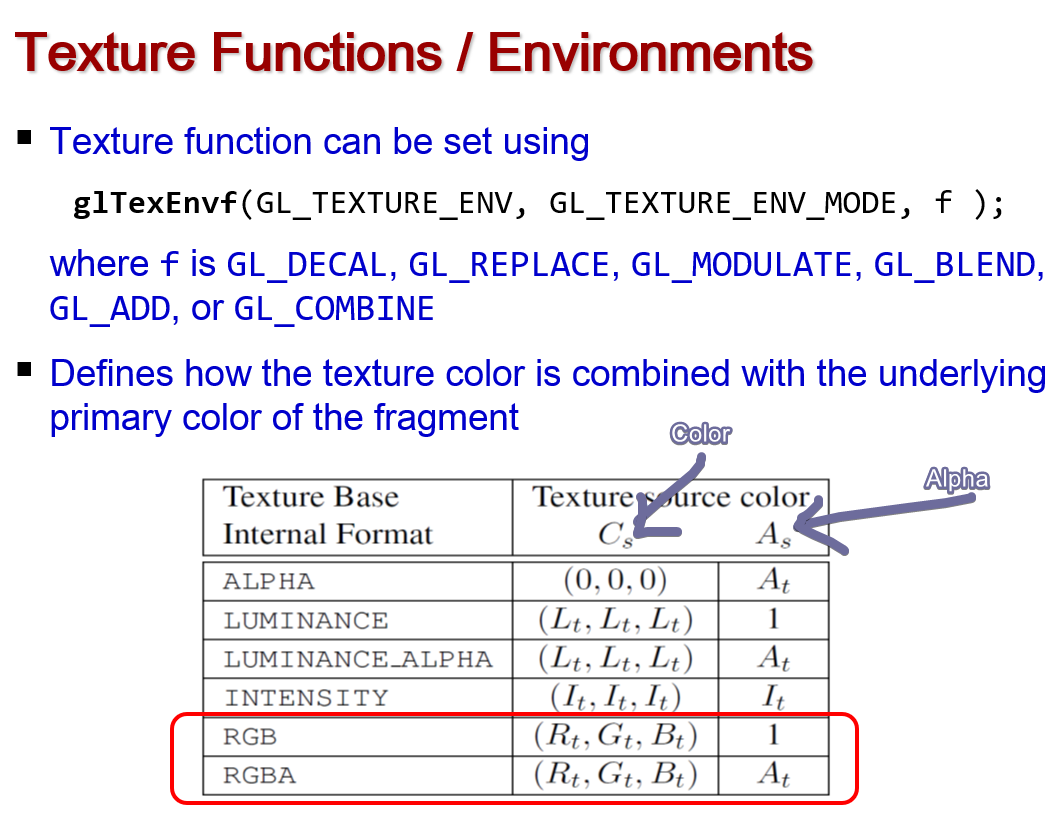
\includegraphics[scale=0.5]{texenv.png}
    \end{center}

\end{frame}

\begin{frame}
    \frametitle{Texture function}

    A \textbf{texture function} acts on the fragment to be textured 
    using the texture image value that applies to the fragment 
    and produces an RGBA color for that fragment. 
    
    \begin{itemize}
        \item C = color (RGB) $\in [0,1]$
        \item A = alpha (A) $\in [0,1]$
        \item $_p$ = color from previous texture stage/incoming fragment
        \item $_s$ = texture source color
        \item $_c$ = texture environment color
        \item $_v$ = final value produced
    \end{itemize}

\end{frame}

\begin{frame}
    \frametitle{Common texture functions}

    \begin{center}
        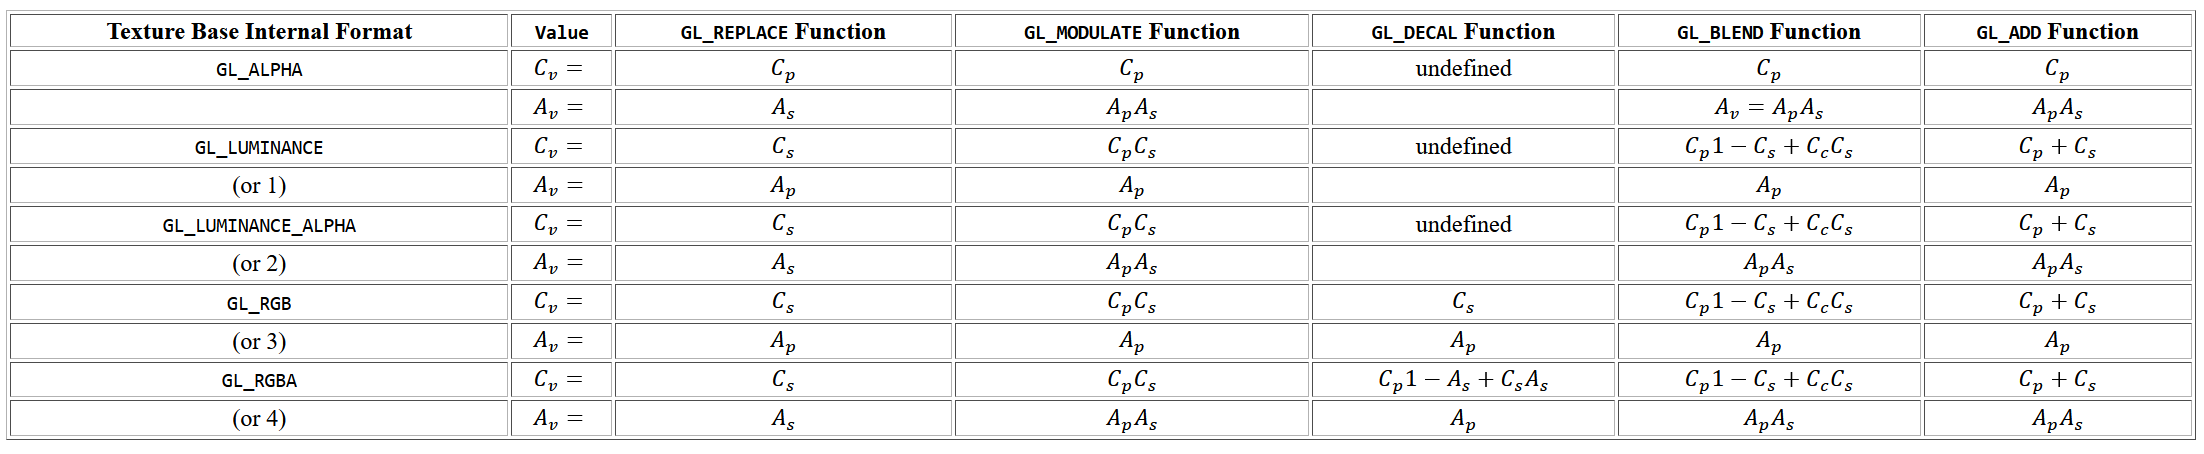
\includegraphics[scale=0.5]{gl-tex-fn.png}
    \end{center}

\end{frame}

\begin{frame}
    \frametitle{Texture wrapping modes}

    \begin{center}
        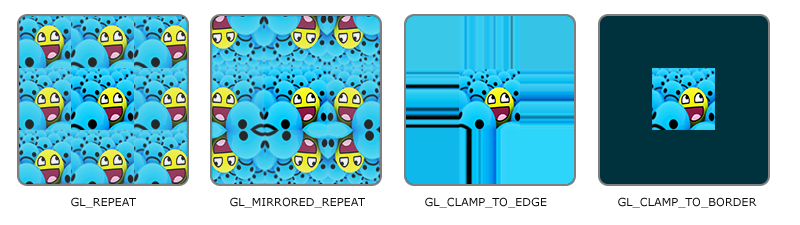
\includegraphics[scale=0.4]{texture_wrapping.png}
        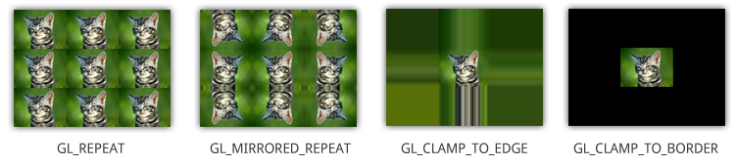
\includegraphics[scale=0.4]{texture_wrapping-1.png}
    \end{center}

\end{frame}

\section{Question 1}

\begin{frame}[plain,standout]
    \AlegreyaExtraBold \LARGE
    Questions
\end{frame}

\begin{frame}
    \frametitle{Question 1}
    Suppose the texture coordinate wrapping mode has been set to \texttt{GL\_REPEAT} 
    for both the $s$ and $t$ texture coordinates. 

    \begin{center}
        
\includegraphics[scale=0.4]{q1.png}
    \end{center}
    
    Given a texture image and a square as shown in the following diagram, 
    what are the 2D texture coordinates assigned to vertices A, B, C and D 
    so that texture-mapped square appears as shown below?
\end{frame}

\begin{frame}
    \frametitle{Question 1}

    \begin{center}
        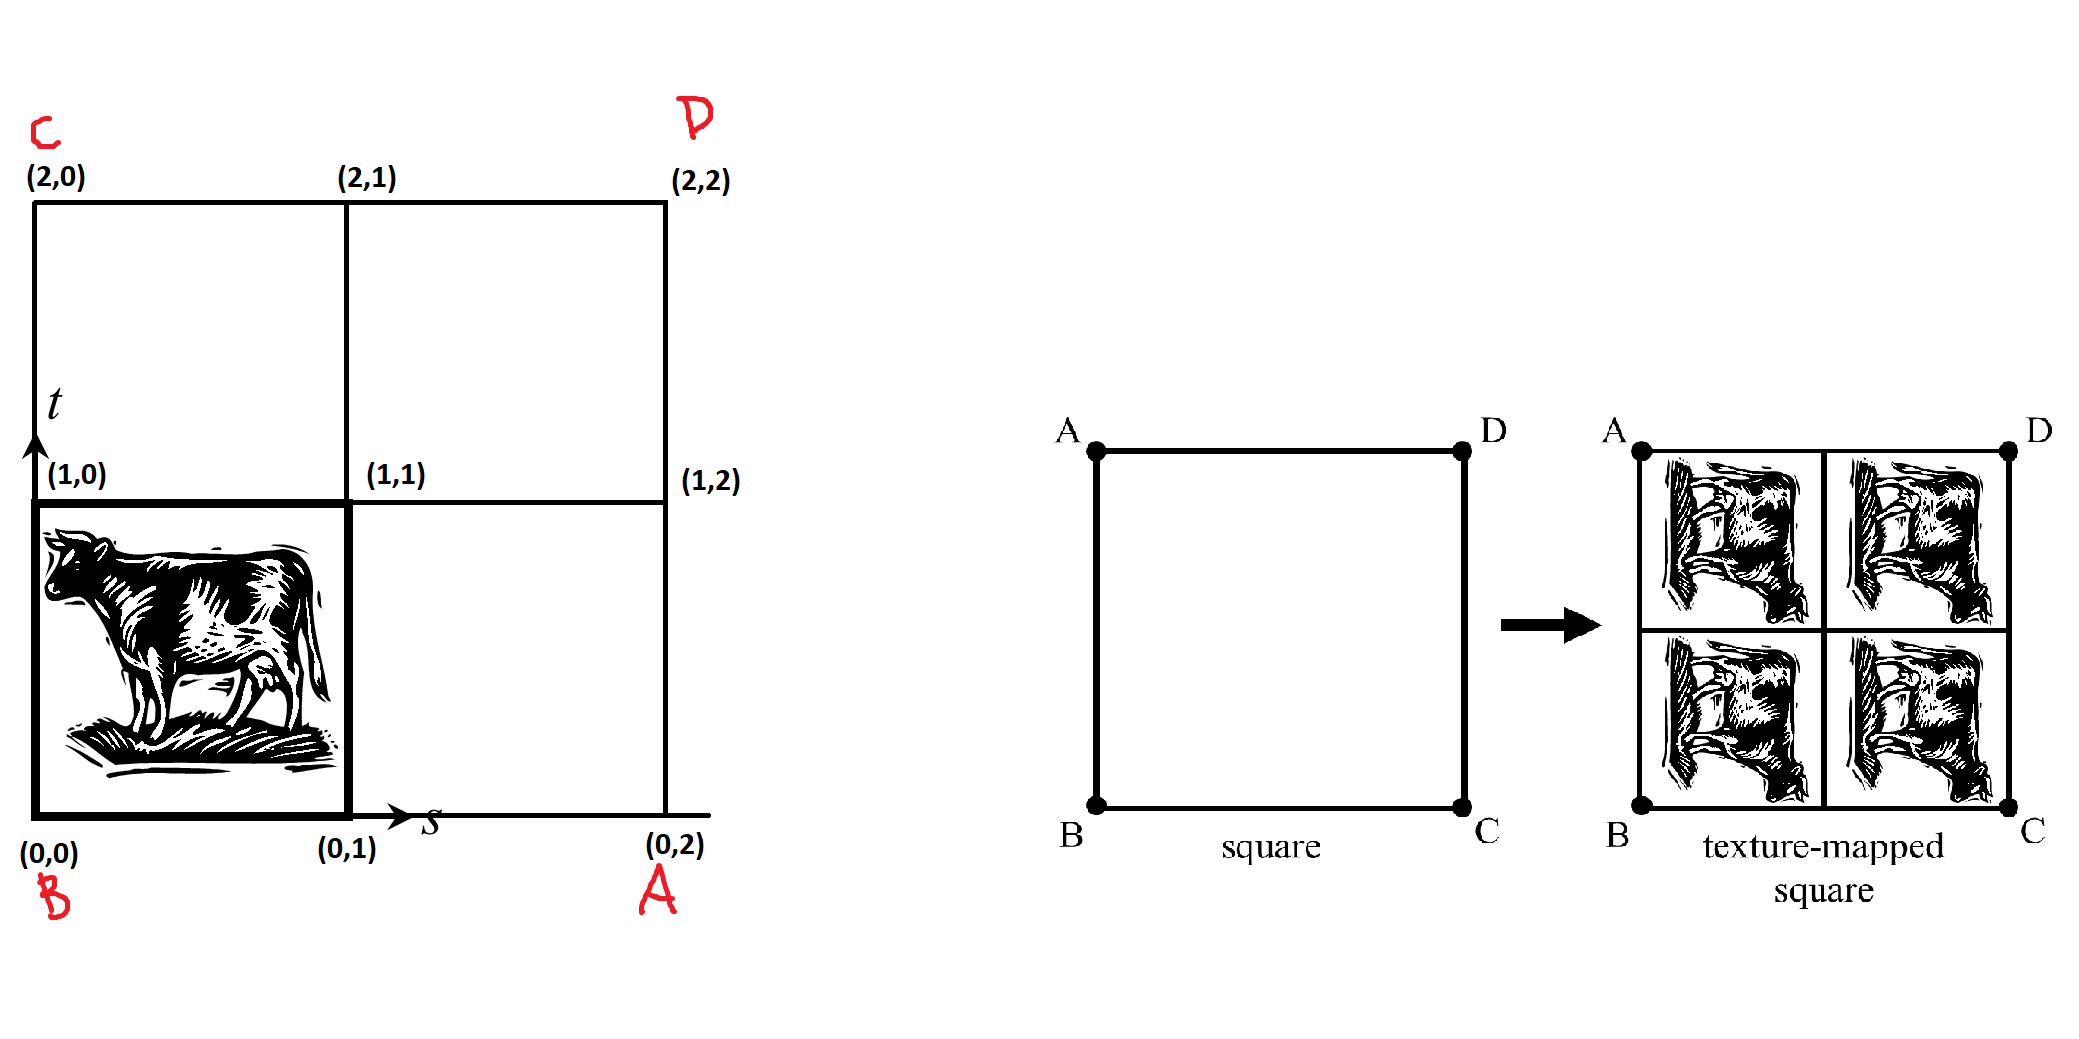
\includegraphics[scale=0.3]{q1-ans.png}
    \end{center}

\end{frame}

\section{Question 2}

\begin{frame}
    \frametitle{Question 2}
    We would like to wrap an entire texture map around the side of the cylinder shown in the diagram. 

    \begin{center}
        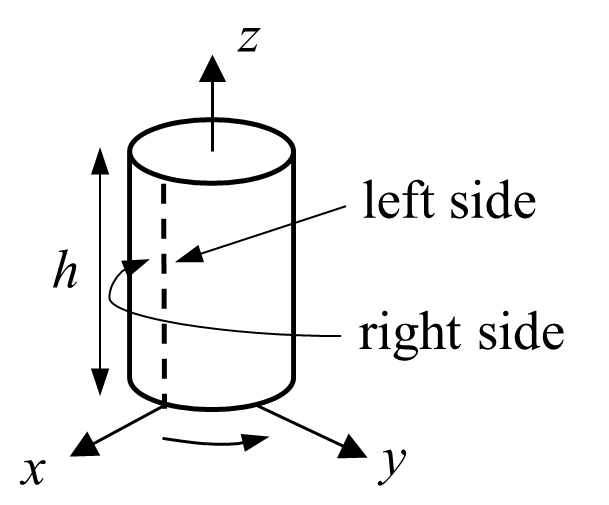
\includegraphics[scale=0.7]{q2.png}
    \end{center}
    
    The center of the base of the cylinder is located at ($0, 0, 0$). 
    Given any point ($p_x, p_y, p_z$) on the side of the cylinder, 
    write the two expressions to compute the $s$ and $t$ texture coordinates at the point. 
    
    \iffalse
    The dashed line in the diagram shows the seam line where the left and right sides of the texture map touches. 
    You are provided with a function angle $(u_x, u_y, v_x, v_y)$, which returns the angle 
    (in the range 0 to 2$\pi$ radians) between the vectors ($u_x, u_y, 0$) and ($v_x, v_y, 0$), 
    measured from vector ($u_x, u_y, 0$) in the counter-clockwise direction about the z-axis.
    \fi

\end{frame}

\begin{frame}
    \frametitle{Question 2}

    Demo!


\end{frame}

\begin{frame}
    \frametitle{Question 2}

    \begin{tcolorbox}
        $s = $ arc length between vector (1,0) and ($p_x, p_y$) $/ 2\pi$ \\
        $t = p_z / h$
    \end{tcolorbox}

    $s \in [0, 1] \mapsto [0, 2\pi]$\\
    $t \in [0, 1] \mapsto [0, h]$\\

\end{frame}

\section{Question 3}

\begin{frame}
    \frametitle{Question 3a}

    \begin{tcolorbox}[colback=teal!5!white]
        \textcolor{teal}{pollev.com/peixian}
    \end{tcolorbox}

    Given a 512 $\times$ 512 texture image, we want to create a mipmap from it and use the appropriate mipmap level 
    during rendering. 

    \vspace{1em}

    How many levels are in the mipmap? (including the original texture level)
\end{frame}

\begin{frame}
    \frametitle{Question 3a}

    \begin{center}
        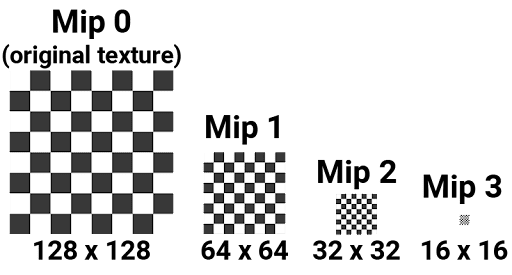
\includegraphics[scale=0.45]{mipmap-levels.png}
    \end{center}

    Mipmap level 0 is original texture. Additionally can halve it's length and width $\log(n)$ times
    (given $n = \min(h,w)$).

    \begin{tcolorbox}
        \centering
        $\log(512) + 1 = 10$
    \end{tcolorbox}

\end{frame}

\begin{frame}
    \frametitle{Question 3b}

    \begin{tcolorbox}[colback=teal!5!white]
        \textcolor{teal}{pollev.com/peixian}
    \end{tcolorbox}

    The mipmap is used to texture-map a 3D square that appears in a 100 $\times$ 100 region on the screen. 
    What is the best integer mipmap level to use to texture-map the square? 
    Assume that we \textit{prefer a more blurred rendered image} if the exact level is not an integer. 

    \vspace{1em}
    
    The highest-resolution texture image is level 0, the next is level 1, and so on.

\end{frame}

\begin{frame}
    \frametitle{Question 3b}

    Manually halving the dimension: 
    512 $\rightarrow$ 256 $\rightarrow$ 128 $\rightarrow$ 64 < 100

    \begin{tcolorbox}
        \centering
        $\lceil \log(512/100) \rceil = \lceil \log(5.12) \rceil = 3$
    \end{tcolorbox}


\end{frame}

\begin{frame}
    \frametitle{Question 3c}

    \begin{tcolorbox}[colback=teal!5!white]
        \textcolor{teal}{pollev.com/peixian}
    \end{tcolorbox}

    Some rendering systems can actually take non-integer mipmap level and compute the result by interpolating between 
    two mipmap levels. (aka \textbf{\textit{Trilinear interpolation}})

    \vspace{1em}
    
    In the case of Part (b), what is the exact mipmap level to use to texture-map the square? Round your answer to 2 decimal places. 
    You can use the formula $\log_2(x) = \log_{10}(x) / \log_{10}(2)$.

\end{frame}

\begin{frame}
    \frametitle{Magnification and Minification}

    \begin{center}
        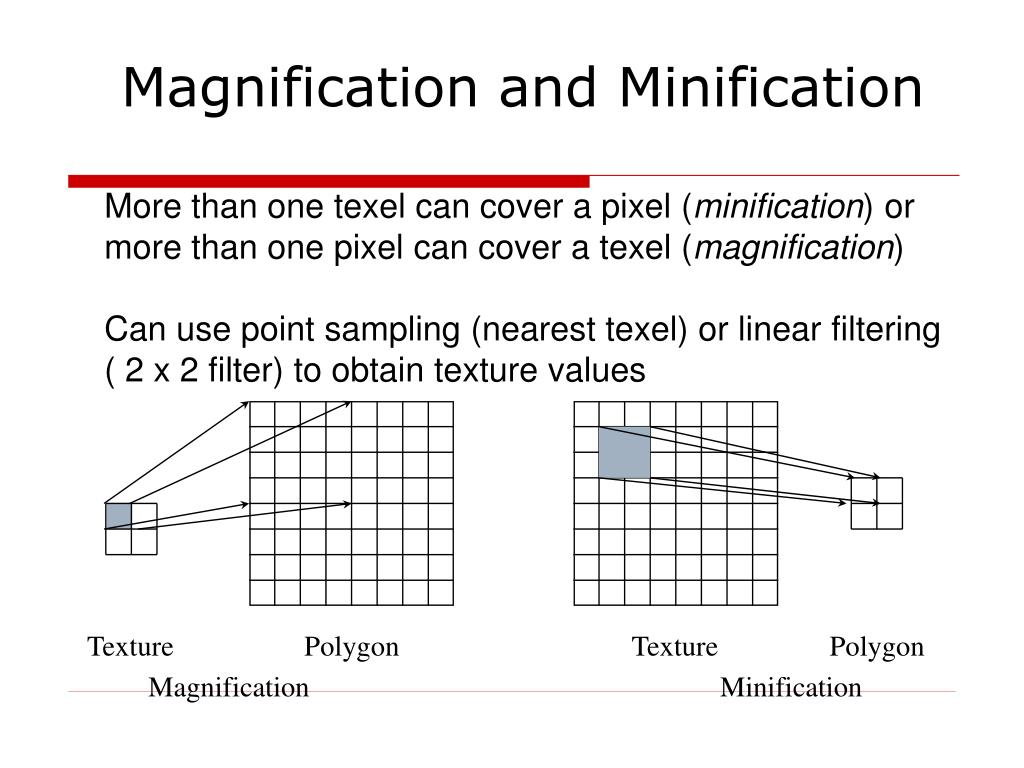
\includegraphics[scale=0.3]{tex_mag-min.jpg}
    \end{center}

\end{frame}

\section{Question 4}

\begin{frame}
    \frametitle{Question 4}

    Given a gray-scale image $I [1 \dots W, 1\dots H]$, we can compute a special table $S[1 \dots W, 1 \dots H]$ such that
    $S[m,n] = \sum_{i=1}^m \sum_{j=1}^n I[i \dots j]$. Then using $S$, the sum of pixel values within
    any rectangular region of the range $I[x_i \dots x_2, y_1 \dots y_2]$ can be computed in constant time:

    \vspace{1em}

    \begin{tcolorbox}
        \begin{equation*} 
            S[x_2, y_2] - S[x_1 - 1, y_2] - S[x_2, y_1 - 1] + S[x_1 - 1, y_1 - 1]
        \end{equation*}
    \end{tcolorbox}
\end{frame}

\begin{frame}
    \frametitle{Summed Area Table}

    \begin{center}
        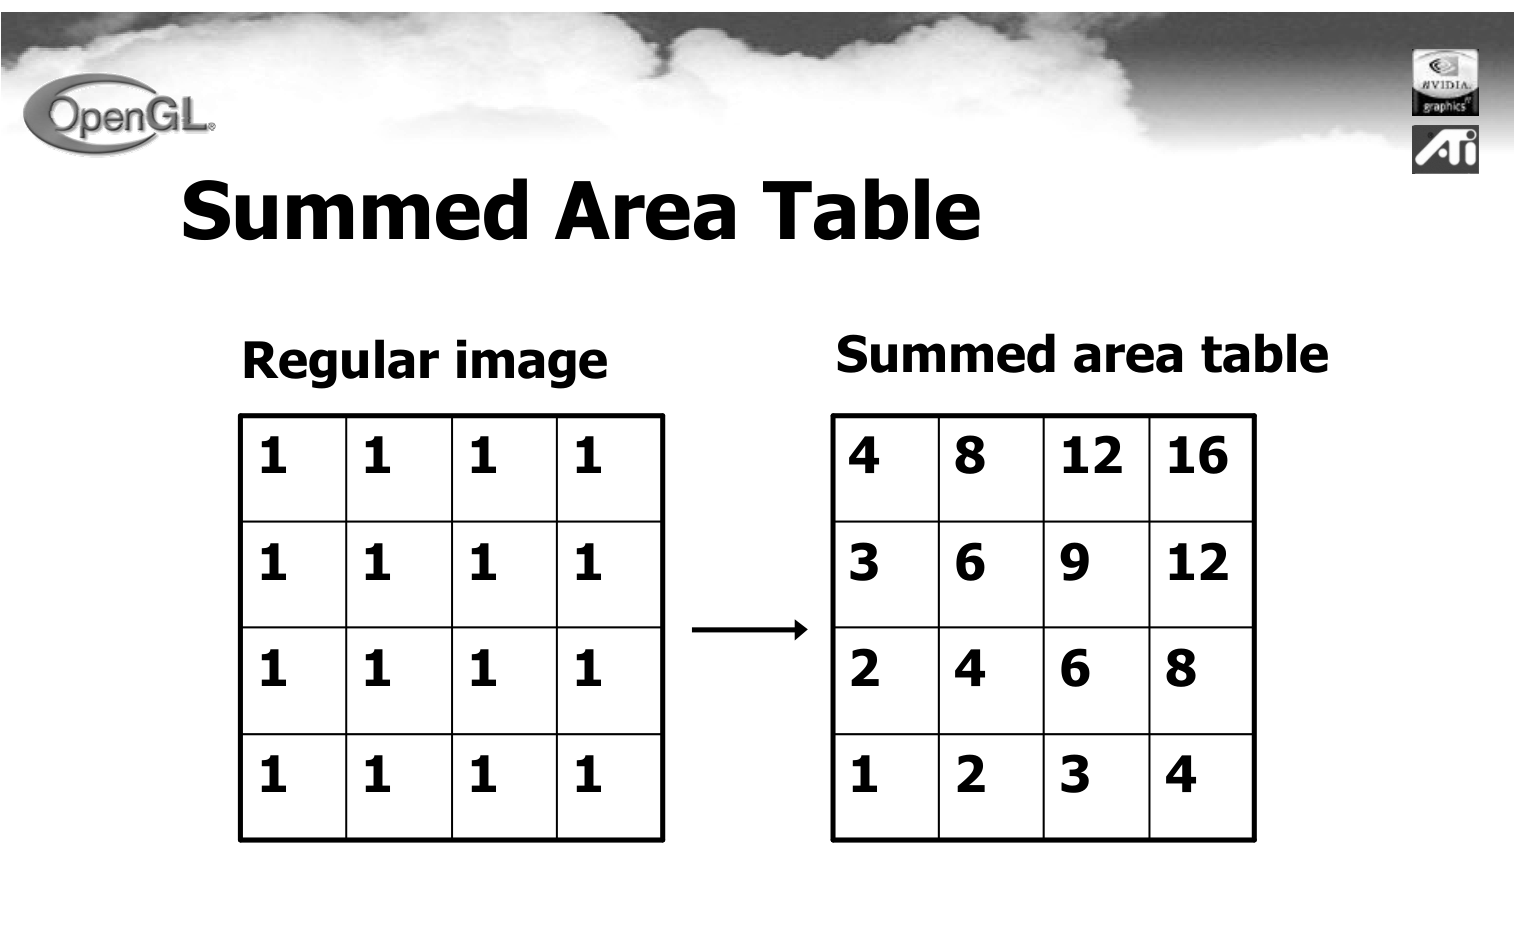
\includegraphics[scale=0.4]{sum-area-table1.png}
    \end{center}

\end{frame}

\begin{frame}
    \frametitle{Summed Area Table}

    \begin{center}
        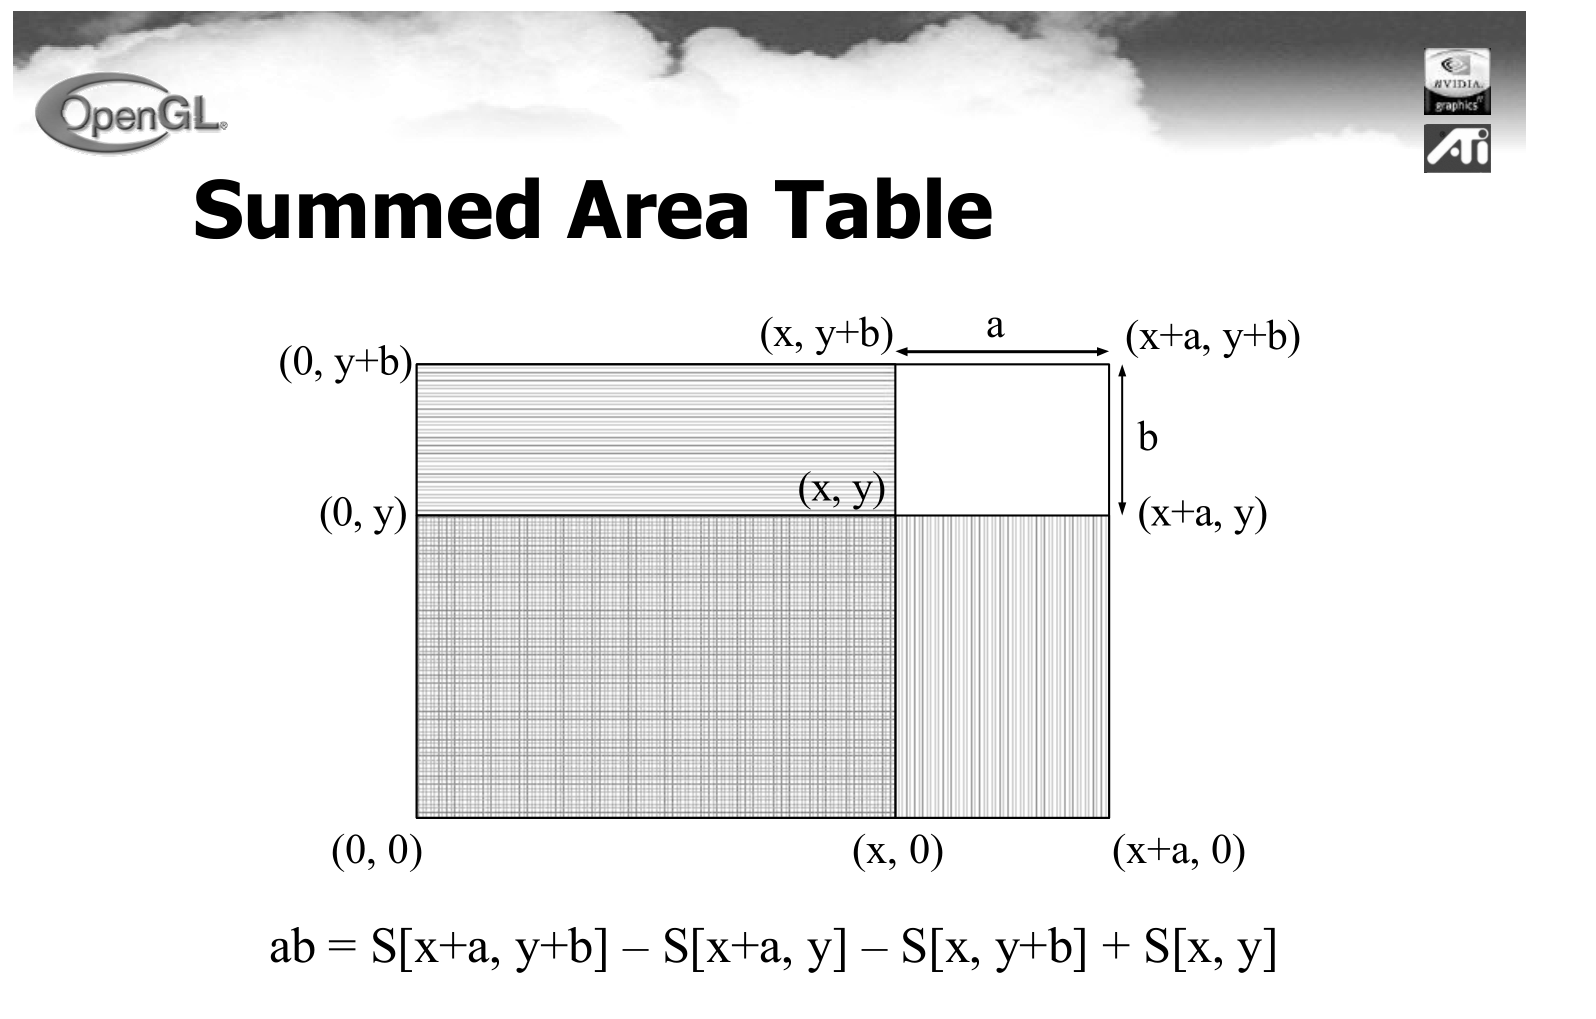
\includegraphics[scale=0.4]{sum-area-table2.png}
    \end{center}

\end{frame}

\begin{frame}
    \frametitle{Question 4a}

    What could be the use of the special table $S$ for overcoming a particular problem in texture mapping?
    Explain why it is suitable.

\end{frame}

\begin{frame}
    \frametitle{Solves \textbf{aliasing}!}

    We can approximate the pre-image of a fragment as a rectangle, 
    and use the special table S to quickly find the average of the
    texel values within the rectangular region. 
    
    \begin{itemize}
        \item efficient area sampling within \textbf{any rectangular region}
        \item S can be precomputed before real-time rendering
    \end{itemize}

\end{frame}

\begin{frame}
    \frametitle{Question 4b}

    Compare the quality of the rendered image produced by the technique you have learned in class, 
    with that using the special table S?  What attributes to the difference?

    \begin{tcolorbox}
        What do we compare Summed Area Table to?
    \end{tcolorbox}

\end{frame}

\begin{frame}
    \frametitle{Quality comparison}

    \begin{tcolorbox}
        Ans: Mipmapping
    \end{tcolorbox}

    The rendered image will look better and sharper
    This is because it can have a \textbf{more accurate approximation} of the pre-image
    region of the fragment (\textbf{arbitrary region in constant time}).

\end{frame}

\section{Question 5}

\begin{frame}
    \frametitle{Question 5a}

    A reflective object can be rendered using reflection mapping or ray tracing. List two situations 
    where there will be obvious differences between the images produced by the two methods.
\end{frame}

\begin{frame}
    \frametitle{Situation 1: Self-intersection}

    The object itself is not part of the environment!

\end{frame}

\begin{frame}
    \frametitle{Situation 2: Relatively large object}

    When the reflective object is quite large compared to the size of its surrounding.
    
    \begin{center}
        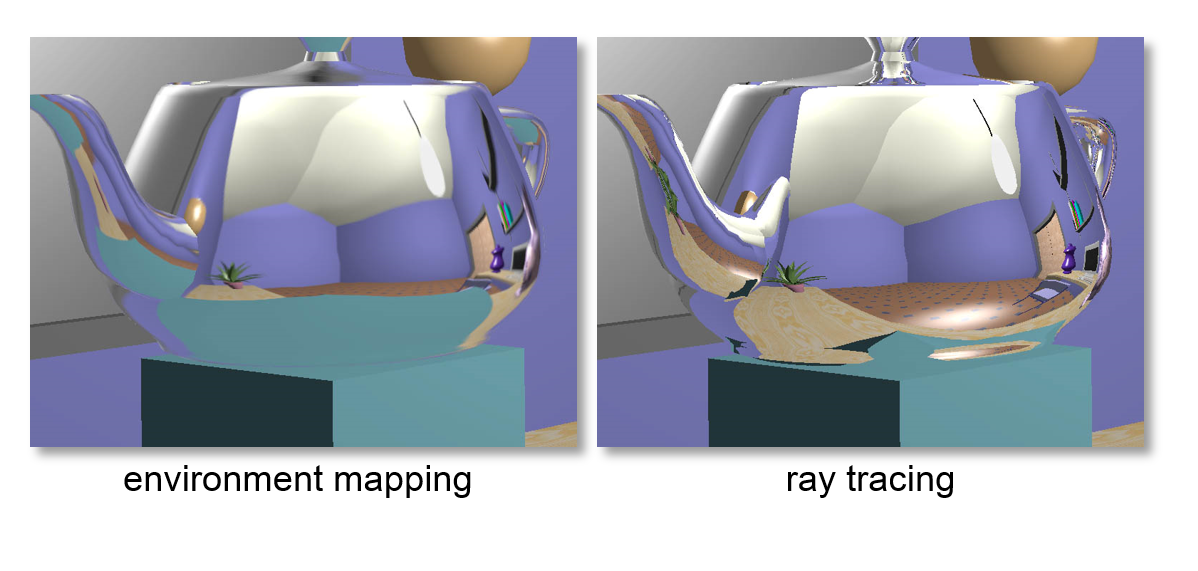
\includegraphics[scale=0.5]{env-inaccuracy.png}
    \end{center}

\end{frame}

\begin{frame}
    \frametitle{Question 5b}

    Describe a way you can use to detect that the features on an object are actually bump-mapped 
    instead of real geometry.

\end{frame}

\begin{frame}
    \frametitle{Question 5c}

    \begin{tcolorbox}[colback=teal!5!white]
        \textcolor{teal}{pollev.com/peixian}
    \end{tcolorbox}

    Suppose you can extend the functionalities in any stage of the raster graphics pipeline. 
    We want to render polygons with bump-mapping. 

    \begin{enumerate}
        \item Should the lighting computation be performed per fragment, per vertex, or per polygon?
        \item At which pipeline stage should the lighting computation be performed?
    \end{enumerate}

\end{frame}

\begin{frame}
    \frametitle{Bump mapping}

    \begin{center}
        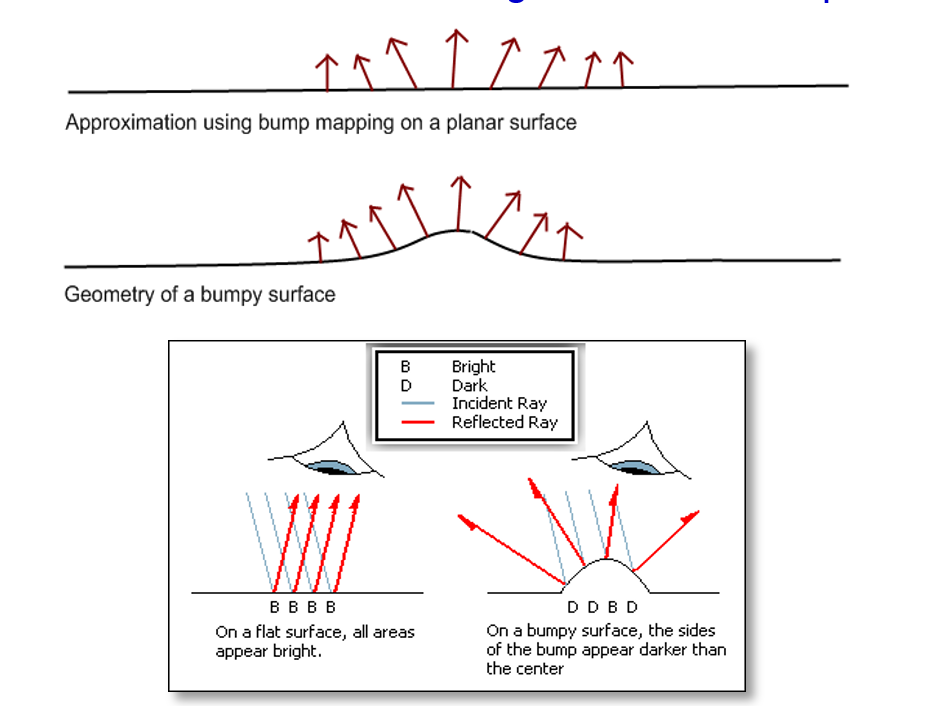
\includegraphics[scale=0.4]{bump-normals.png}
    \end{center}

    Normals provided by the bump map \textbf{per fragment} to do lighting computation with
    (e.g. Phong Illumination Equation).

\end{frame}

\begin{frame}
    \frametitle{Lighting computation}

    Probably in the fragment processing stage

    \begin{center}
        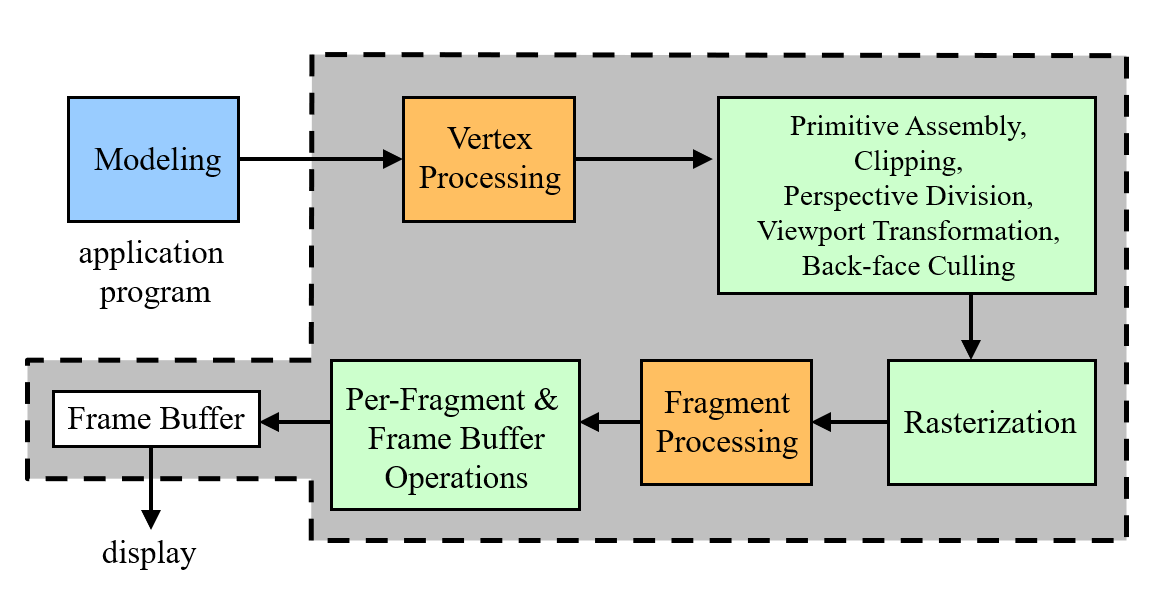
\includegraphics[scale=0.5]{pipeline.png}
    \end{center}

\end{frame}

\begin{frame}
    \frametitle{Question 5d}

    \begin{tcolorbox}[colback=teal!5!white]
        \textcolor{teal}{pollev.com/peixian}
    \end{tcolorbox}

    In a virtual outdoor scene, each tree is rendered using a vertical rectangular billboard. 
    The vertical axis of the world is the z-axis. The viewpoint is at ($v_x, v_y, v_z$). 
    For a billboard whose center is at ($b_x, b_y, b_z$), what should be the normal vector of the billboard rectangle? 
    You need not normalize the vector.

\end{frame}

\begin{frame}
    \frametitle{Question 5d}

    \begin{center}
        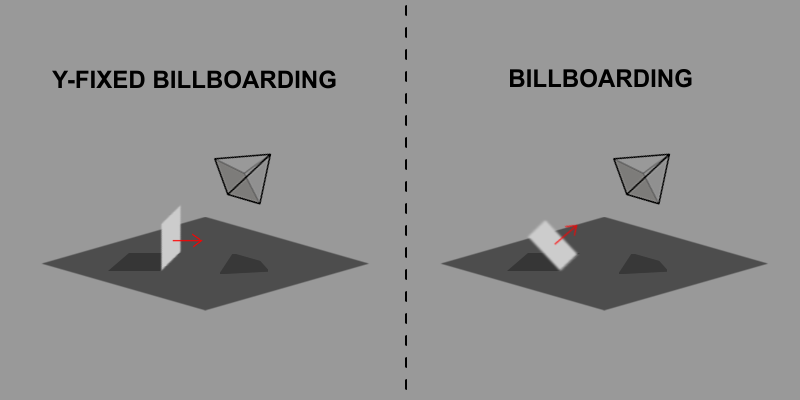
\includegraphics[scale=0.35]{billboarding.png}
    \end{center}

    \begin{tcolorbox}
        \begin{itemize}
            \item z-axis is fixed: $(v_x - b_x, v_y - b_y, 0)$
            \item completely billboarded: $(v_x - b_x, v_y - b_y, v_z - b_z)$
        \end{itemize}
    \end{tcolorbox}

\end{frame}

\begin{frame}[plain,standout]
    \AlegreyaExtraBold \LARGE
    Attendance taking
\end{frame}

\ThankYou
\begin{frame}[plain,standout]
    Thanks! Get the slides here after the tutorial.\\
    \vspace{2em}
    \scalebox{3}{\faGithub}\par\bigskip
    \url{https://trxe.github.io/cs3241-notes}
\end{frame}

\end{document}